\documentclass{article}
\pagenumbering{gobble}
\usepackage{tikz}
\usetikzlibrary{matrix,chains,positioning,decorations.pathreplacing,arrows}
\usepackage{calc}
\begin{document}

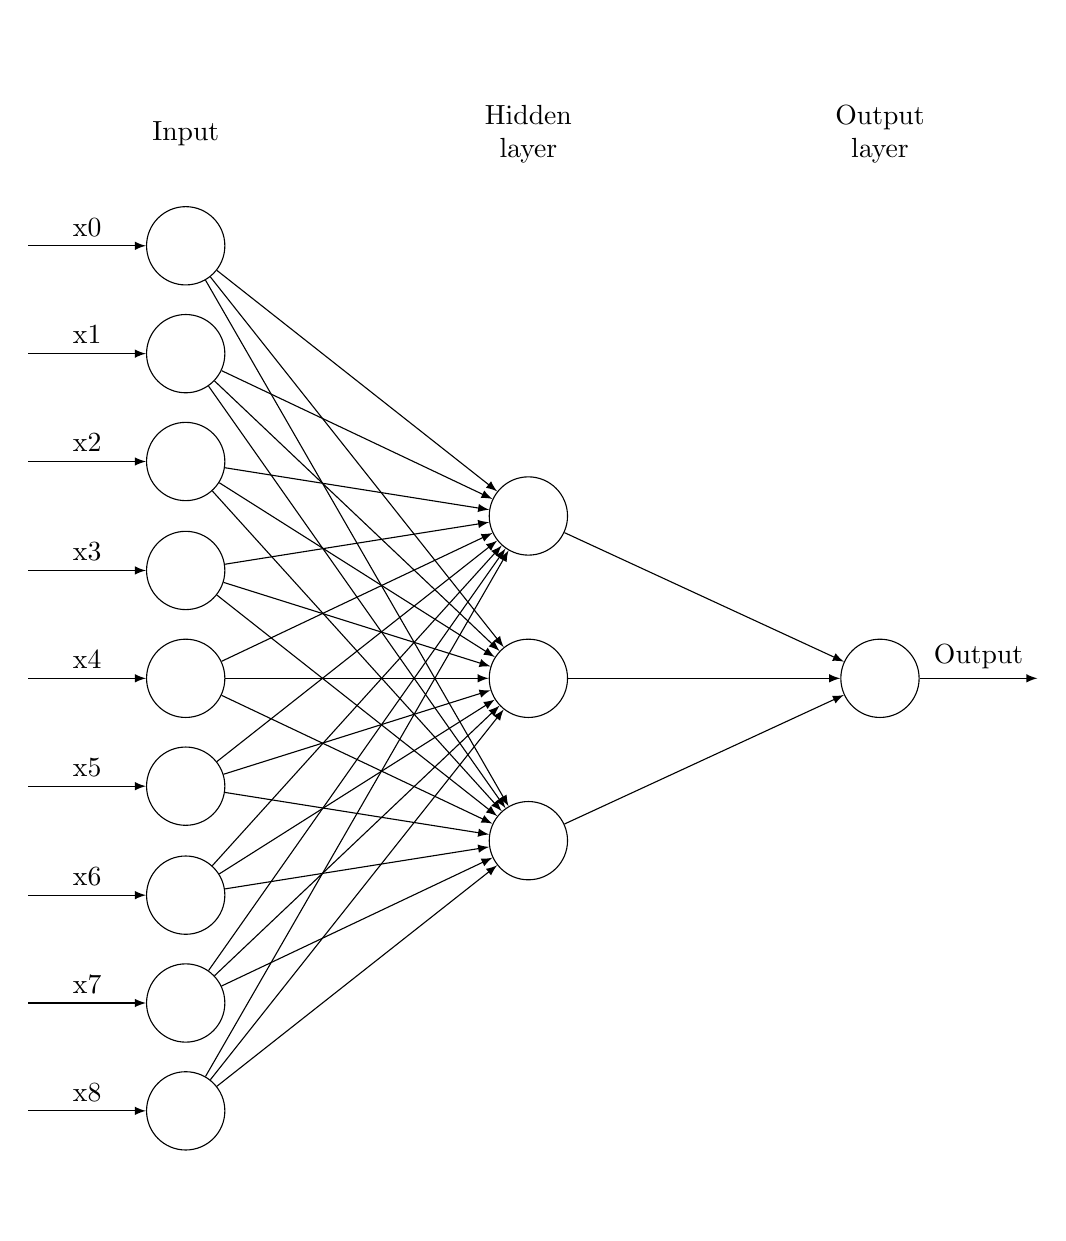
\begin{tikzpicture}[
plain/.style={
  draw=none,
  fill=none,
  },
net/.style={
  matrix of nodes,
  nodes={
    draw,
    circle,
    inner sep=10pt
    },
  nodes in empty cells,
  column sep=2cm,
  row sep=-9pt
  },
>=latex
]
\matrix[net] (mat)
{
|[plain]| \parbox{1.3cm}{\centering Input} & |[plain]| \parbox{1.3cm}{\centering Hidden\\layer} & |[plain]| \parbox{1.3cm}{\centering Output\\layer} \\
          & |[plain]| & |[plain]| \\
|[plain]| & |[plain]| & |[plain]| \\
          & |[plain]| & |[plain]| \\
|[plain]| & |[plain]| & |[plain]| \\
          & |[plain]| & |[plain]| \\
|[plain]| &           & |[plain]| \\
          & |[plain]| & |[plain]| \\
|[plain]| & |[plain]| & |[plain]| \\
          &           &           \\
|[plain]| & |[plain]| & |[plain]| \\
          & |[plain]| & |[plain]| \\
|[plain]| &           & |[plain]| \\
          & |[plain]| & |[plain]| \\
|[plain]| & |[plain]| & |[plain]| \\
          & |[plain]| & |[plain]| \\
|[plain]| & |[plain]| & |[plain]| \\
          & |[plain]| & |[plain]| \\
|[plain]| & |[plain]| & |[plain]| \\};

\foreach \ai [count=\mi from 0] in {2,4,...,18}
  \draw[<-] (mat-\ai-1) -- node[above] {x{\mi}} +(-2cm,0);
\foreach \ai in {2,4,...,18}
{\foreach \aii in {7,10,13}
  \draw[->] (mat-\ai-1) -- (mat-\aii-2);
}
\foreach \ai in {7,10,13}
  \draw[->] (mat-\ai-2) -- (mat-10-3);
\draw[->] (mat-10-3) -- node[above] {Output} +(2cm,0);

\end{tikzpicture}

\end{document}